\section{Demonstrator Prototype}
\label{sec:design}

In this project, several software technologies were used that have already been mentioned and described in section above. For all technologies to communicate with each other, a REST API is used. User can view the application by sending HTTP request to server from web browser and server replying with a handled response. A user has different "interaction" he/she can do with the web application, those are described in Section~\ref{sub:usecase}.

\subsection{Architecture}
\label{sub:architeure}
Figure~\ref{fig:archdiagram} represents the architecture diagram for the FeedApp.
A Client (user) uses the web browser to send requests and get responses from the server (application). To use the application the user needs to be authenticated (logged in), at least for the most use cases of the application. Requests gets handled by the REST API on the server which processes the request and sends a response accordingly. REST API communicates with the database to save/get persisted data.

There is also support for IoT devices to communicate with the server, and it sends the requests straight to the REST API which doesn't have to go through the extra steps with authentication and Model view in web browser.

This project additionally includes a messaging system that gets poll information from REST API and sends them to a NoSQL database. Where the polls can be used in other use cases, than the web application intends to.
\begin{figure}[H]
  \centering
  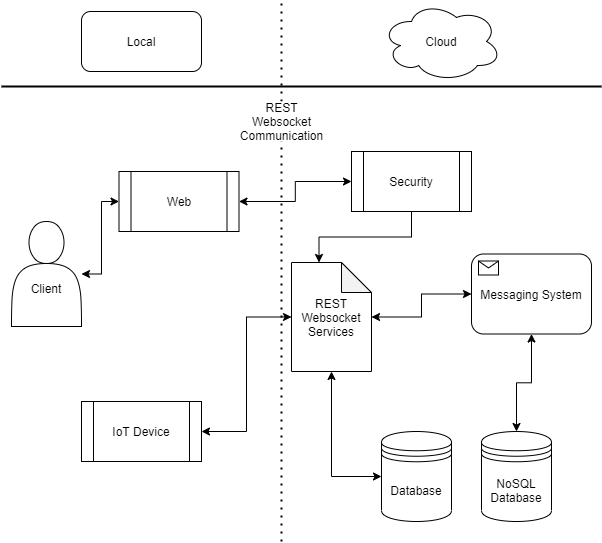
\includegraphics[scale=0.5]{figs/archdiagram.png}
  \caption[scale=0.5]{Architecture diagram.}
  \label{fig:archdiagram}
\end{figure}

\subsection{Application flow}
\label{sub:appflow}
Application flow can be seen in Figure~\ref{fig:applicationflow}, which has the thought out interactions on the different web pages and what will be possible for the user to do. A users will be able to vote on a public poll without the need of being authenticated, or be in possession of an account at all. If the poll is private, then the user will be able to create an account to vote. After creating an account, user will have the opportunity to create/edit his/her own polls. User needs a PollID to vote, and to find the different PollIDs, an option to search for available polls by their respective names will be created. 

Some actions can end in a failure, these will be handled with proper responses giving the user "detailed" information on what to correct, for the different actions.
\begin{figure}[H]
  \centering
  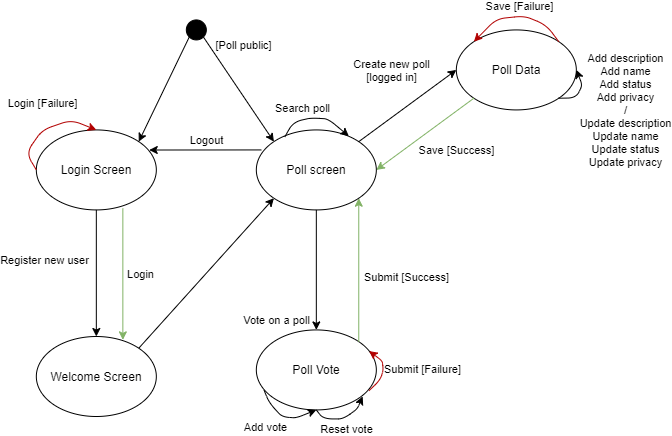
\includegraphics[scale=0.5]{figs/applicationflow.png}
  \caption[scale=0.5]{Application flow.}
  \label{fig:applicationflow}
\end{figure}

\subsection{Use case}
\label{sub:usecase}
In Figure~\ref{fig:usecases}, user enters the Application via web browser and is able to login or register new account. On main page after logging in; user can create a new poll, delete or edit an already existing poll (if user is owner), search/look-up a poll and vote on it. Since the application also supports IoT devices, the use case of an IoT device is to enter a poll with PollID and vote on it.

\begin{itemize}
  \item \textbf{Vote on a Poll:} Everyone can vote on a public poll, using a web form, but to vote on a private poll the user must be logged in.
  \item \textbf{Register:} Everyone can register a new account to use the web application services, using OAuth.
  \item \textbf{Create Poll:} A logged in user can create a new poll using a web form.
  \item \textbf{Subscribe to Poll:} A logged in user can subscribe to a poll after entering the voting screen with PollID.
  \item \textbf{Show own polls:} A logged in user can view his/her own created polls, including the "live" voting results.
  \item \textbf{Show subscription messages:} A logged in user can view messages from subscriptions, on subscribed polls.
  \item \textbf{Delete Poll:} A logged in user can delete own polls from show own polls screen.
  \item \textbf{Edit Poll:} A logged in user can edit his/her own polls, using another web form from show own polls screen.
  \item \textbf{Look-up a Poll:} Everyone can look-up a public poll by the name, but only logged in users can look-up private polls.
  \item \textbf{IoT Device:} An IoT device can vote on all polls with known PollID. IoT can also see Poll data, with-it the results as well.
\end{itemize}
\begin{figure}[H]
  \centering
  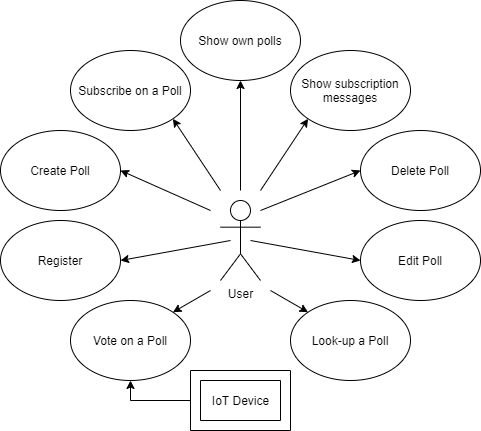
\includegraphics[scale=0.5]{figs/usecases.png}
  \caption[scale=0.5]{Use cases.}
  \label{fig:usecases}
\end{figure}

\subsection{Domain model}
\label{sub:domainmodel}
The domain model in Figure~\ref{fig:domainmodel} describes the planned persisted entities. A User with a uID as primary key can have multiple Polls, with a PollID as primary key and User as a foreign key. The database will also save which user has voted on which poll, so that a logged in user cannot vote multiple times on the same poll. This data is persisted into "User has Voted" table.
\begin{figure}[H]
  \centering
  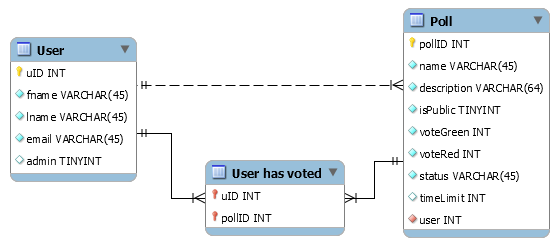
\includegraphics[scale=0.5]{figs/domainmodel.png}
  \caption[scale=0.5]{Domain model.}
  \label{fig:domainmodel}
\end{figure}

The user also has lists of Polls he/she subscribed to, to receive updates, and subscription message list, with messages from the subscriptions.

\par\noindent In the next section implementation of the project will be covered, and the different technologies used.